\section{The bias-variance tradeoff}
\label{sec:bias-variance}

The bias-variance tradeoff is less an algorithm than a \emph{theorem}: a simple
and very general decomposition of the test error of any learning procedure into
three interpretable pieces. It explains, quantitatively, why both overly simple
and overly complex models generalise poorly, and it is the cleanest way to think
about the role of model complexity and of regularisation.

\subsection{Setup: a probabilistic model of the data}

We place ourselves in the regression setting, but now we take seriously the fact
that the data is \emph{random}. We assume there is a ground-truth function
$f^\star : \R^d \to \R$ and that the labels are noisy observations of it:
\[
y_i = f^\star(x_i) + \varepsilon_i, \qquad
\varepsilon_i \perp x_i, \qquad
\E[\varepsilon_i] = 0, \qquad
\Var(\varepsilon_i) = \sigma^2 .
\]
Here $\varepsilon_i$ is an \emph{irreducible noise}, independent of the input and
centred, with variance $\sigma^2$. Both inputs and labels are random: we write
$(x, y) \sim P_{x,y}$ for a generic data point drawn from this distribution.

A \emph{learning procedure} is a map that turns a training dataset into a
predictor. It first fits a parameter, and then returns the associated function:
\[
\underbrace{\mathcal{D} = \big( (x_1, y_1), \dots, (x_n, y_n) \big)}_{\text{dataset, in } (\R^d \times \R)^n}
\ \longmapsto \
\underbrace{\hat w}_{\text{fitted parameter, in } \R^d}
\ \longmapsto \
\underbrace{f_{\hat w}}_{\text{predictor, in } \F} ,
\]
where $\hat w$ is typically the (possibly regularised) empirical risk minimiser
\[
\hat w \in \argmin_{w} L(w)
\qquad \text{or} \qquad
\hat w = \argmin_{w} \Big\{ L(w) + \frac{\lambda}{2} \Vert w \Vert^2 \Big\} ,
\]
the second being exactly the ridge objective $L_\lambda$ of \Cref{subsec:ridge}, with
the same convention for the constants. Note the difference between the two symbols:
the ridge minimiser is unique, so ``$=$'' is legitimate, whereas the unregularised
minimiser need not be, whence ``$\in$''. When it is not unique, the rule used to pick
one of them (for us, the minimum-norm rule) is part of the learning procedure and
must be specified; this will matter a great deal in \Cref{subsec:double-descent}.
The crucial point, and the whole source of the ``variance'' below, is that the
trained predictor $\hat f := f_{\hat w}$ \emph{depends on the random training set}
$\mathcal{D}$: draw a new dataset and you get a different predictor. We write
$\bar f(x) := \E_{\mathcal{D}}[\hat f(x)]$ for the \emph{average predictor},
averaged over the draw of the training data.

\subsection{The one identity behind everything}

The entire decomposition rests on a single elementary fact about squared errors.

\begin{lemma}[Bias-variance identity]
\label{lem:bv-identity}
For any random vector $Z$ with values in $\R^m$ and any constant $c \in \R^m$,
\[
\E\big[ \Vert Z - c \Vert^2 \big] = \E\big[ \Vert Z - \E[Z] \Vert^2 \big]
+ \big\Vert \E[Z] - c \big\Vert^2 .
\]
For $m = 1$ the first term on the right is $\Var(Z)$, which is the only case we need
until \Cref{subsec:kmeans}.
\end{lemma}

\begin{proof}
Introduce $\E[Z]$ and expand:
\begin{align*}
\E\big[\Vert Z - c \Vert^2\big]
&= \E\Big[ \big\Vert (Z - \E[Z]) + (\E[Z] - c) \big\Vert^2 \Big] \\
&= \E\big[\Vert Z - \E[Z] \Vert^2\big]
 + \big\Vert \E[Z] - c \big\Vert^2
 + 2 \big\langle \E[Z] - c,\ \underbrace{\E\big[Z - \E[Z]\big]}_{= \, 0} \big\rangle .
\end{align*}
The cross term vanishes because $\E[Z] - c$ is a constant vector and
$\E[Z - \E[Z]] = 0$.
\end{proof}

\subsection{Peeling off the irreducible noise}

Fix once and for all a test input $x_0$, and let $y = f^\star(x_0) + \varepsilon$ be
the label we would observe there. Two independent sources of randomness are now in
play, and it is worth naming them: the training set $\mathcal{D}$, which decides
$\hat f$, and the test noise $\varepsilon$, which decides $y$. We write
$\E := \E_{\mathcal{D}, \varepsilon}$ for the average over both. Inserting the ground
truth $f^\star(x_0)$ and expanding,
\[
\E\big[(y - \hat f(x_0))^2\big]
= \E\Big[ \big( \underbrace{y - f^\star(x_0)}_{= \, \varepsilon}
  + f^\star(x_0) - \hat f(x_0) \big)^2 \Big] .
\]
Expanding the square gives three terms,
\begin{align*}
\E\big[(y - \hat f(x_0))^2\big]
&= \underbrace{\E\big[(y - f^\star(x_0))^2\big]}_{\text{(I)}}
+ \underbrace{\E\big[(f^\star(x_0) - \hat f(x_0))^2\big]}_{\text{(II)}} \\
&\qquad + 2\, \underbrace{\E\big[(y - f^\star(x_0))(f^\star(x_0) - \hat f(x_0))\big]}_{\text{(III)}} .
\end{align*}
We treat them one by one.
\begin{itemize}
    \item \textbf{(I) is the noise floor.} Since $y - f^\star(x_0) = \varepsilon$,
    term (I) equals $\E[\varepsilon^2] = \sigma^2$.
    \item \textbf{(III) vanishes.} The test noise $\varepsilon$ is independent of the
    training set $\mathcal{D}$ (hence of $\hat f$), and it is centred. Therefore the
    expectation factorises:
    \[
    \E\big[\varepsilon \cdot (f^\star(x_0) - \hat f(x_0))\big]
    = \underbrace{\E[\varepsilon]}_{= \, 0} \cdot
      \E_{\mathcal{D}}\big[f^\star(x_0) - \hat f(x_0)\big] = 0 .
    \]
\end{itemize}
Term (II) no longer involves $\varepsilon$ at all, so the error splits cleanly as
\[
\E\big[(y - \hat f(x_0))^2\big]
= \sigma^2 + \E_{\mathcal{D}}\big[(\hat f(x_0) - f^\star(x_0))^2\big] .
\]
The first term is the \emph{irreducible error}: no procedure can beat it, because it
comes from the noise on the labels themselves. Everything we can hope to control
sits in the second term.

\subsection{Splitting the rest into bias and variance}

It remains to understand $\E_{\mathcal{D}}[(\hat f(x_0) - f^\star(x_0))^2]$, in which
only the training set is random. Apply the
identity of \Cref{lem:bv-identity} with the random variable $Z = \hat f(x_0)$
(random through $\mathcal{D}$) and the constant $c = f^\star(x_0)$ (the ground truth
at $x_0$ is not random). Recalling $\bar f(x_0) = \E_{\mathcal{D}}[\hat
f(x_0)]$,
\[
\E_{\mathcal{D}}\big[(\hat f(x_0) - f^\star(x_0))^2\big]
= \underbrace{\E_{\mathcal{D}}\big[(\hat f(x_0) - \bar f(x_0))^2\big]}_{\text{variance}}
+ \underbrace{\big(\bar f(x_0) - f^\star(x_0)\big)^2}_{\text{bias}^2} .
\]
Equivalently, expanding around $\bar f(x_0)$ directly, the cross term
$2\,\E[(\hat f(x_0) - \bar f(x_0))]\,(\bar f(x_0) - f^\star(x_0))$ is zero
because $\E_{\mathcal{D}}[\hat f(x_0) - \bar f(x_0)] = 0$ and $\bar f(x_0) -
f^\star(x_0)$ is not random. Putting the two decompositions together yields the main
result.

\begin{thm}[Bias-variance decomposition]
Under the model above, the expected squared error at a test input $x_0$ decomposes as
\[
\E_{\mathcal{D}, \varepsilon}\big[(y - \hat f(x_0))^2\big]
= \underbrace{\sigma^2}_{\text{noise}}
+ \underbrace{\big(\bar f(x_0) - f^\star(x_0)\big)^2}_{\text{bias}^2(x_0)}
+ \underbrace{\E_{\mathcal{D}}\big[(\hat f(x_0) - \bar f(x_0))^2\big]}_{\text{variance}(x_0)} .
\]
Averaging over the test input $x_0 \sim P_x$ gives the same decomposition for the
overall test error, with $\mathrm{bias}^2$ and $\mathrm{variance}$ averaged over
$x_0$.
\end{thm}

\subsection{Reading the three terms}

The three pieces have clear and distinct meanings.
\begin{itemize}
    \item \textbf{Noise $\sigma^2$.} The irreducible error, coming from the label
    noise. It is a property of the data, not of the model, and no learning
    procedure can go below it.
    \item \textbf{Bias $\bar f(x_0) - f^\star(x_0)$.} How far the \emph{average}
    predictor is from the truth. A large bias means the model is systematically
    wrong, typically because the model class is too rigid to represent $f^\star$
    (\emph{underfitting}). Simple models (e.g.\ a low-degree polynomial) have high
    bias.
    \item \textbf{Variance $\E[(\hat f(x_0) - \bar f(x_0))^2]$.} How much the
    predictor wobbles when the training set changes. A large variance means the model
    is very sensitive to the particular data it saw (\emph{overfitting}). Flexible,
    high-capacity models (e.g.\ a high-degree polynomial) have high variance.
\end{itemize}

\paragraph{What the bias really measures.}
The bias is the term students most often get wrong, because ``the average predictor''
sounds like something one would have to simulate. For the procedures of these notes it
is not: it is simply what the procedure returns when you hand it \emph{noiseless}
labels. The reason is that least squares, ridge and polynomial interpolation are all
\emph{linear in $y$}.

\begin{prop}[Bias of a linear procedure]
\label{prop:bias-linear}
Fix the inputs $x_1, \dots, x_n$ (deterministic design), so that the only randomness in
the training set is the noise $\varepsilon = (\varepsilon_1, \dots, \varepsilon_n)$.
Suppose the fitted predictor depends linearly on the labels, i.e.\ $\hat f =
\mathcal{A}(y)$ for some linear map $\mathcal{A} : \R^n \to \F$. Then
\[
\bar f = \E_{\mathcal{D}}\big[ \mathcal{A}(y) \big] = \mathcal{A}\big( \E[y] \big)
= \mathcal{A}\big( f^\star(x_1), \dots, f^\star(x_n) \big) .
\]
In words: \emph{the average predictor is the one the same procedure would have produced
from noiseless data}. Consequently the bias is a pure \emph{approximation error},
measuring how well the procedure reconstructs $f^\star$ from its values at the design
points, and it does not involve $\sigma^2$ at all.
\end{prop}

\begin{proof}
Linearity of $\mathcal{A}$ lets it commute with the expectation, and $\E[y_i] =
f^\star(x_i) + \E[\varepsilon_i] = f^\star(x_i)$ since the noise is centred.
\end{proof}

This applies to every procedure we have met: $\hat w = (X^\top X)^{-1} X^\top y$ is
linear in $y$, so is the ridge estimator $(X^\top X + n\lambda I)^{-1} X^\top y$, so is
the minimum-norm interpolant $X^\top (XX^\top)^{-1} y$, and so is Lagrange
interpolation. It does \emph{not} apply to a neural network, whose dependence on $y$ is
anything but linear, and there the bias really is a subtler object.

\paragraph{The two extremes.}
The decomposition is easiest to feel on the two caricatural procedures sitting at
either end of the complexity axis. Take a scalar input and the polynomial feature map
$\phi^{(k)}(x) = (1, x, \dots, x^k)$ of \Cref{subsec:features}.

\emph{Degree $k = 0$: predict the mean.} Here $\F$ contains only the constant
functions, and the fitted predictor is $\hat f \equiv \bar y = \tfrac1n \sum_i y_i$,
whatever the shape of the data.
\begin{itemize}
    \item \emph{Variance $\approx 0$.} Redrawing the noise barely moves $\bar
    y$: since the $y_i$ are averaged, $\Var(\bar y) = \sigma^2/n$, which
    is small. The predictor is almost the same function every time.
    \item \emph{Bias: everything.} By \Cref{prop:bias-linear} the average predictor
    is constant, equal to the mean of the \emph{truth} over the design points,
    $\bar f \equiv \tfrac1n \sum_i f^\star(x_i)$. The bias at $x_0$ is therefore
    $\tfrac1n\sum_i f^\star(x_i) - f^\star(x_0)$, as large as the variation of
    $f^\star$ itself. Unless the
    truth really is constant, this procedure is systematically wrong, and no amount of
    extra data will help.
\end{itemize}

\emph{Degree $k = n-1$: interpolate.} Here $d = n$, and by Lagrange interpolation
there is exactly one polynomial passing through all $n$ points, so $\hat f(x_i) =
y_i$ for every $i$ and the training error is zero.
\begin{itemize}
    \item \emph{Variance: enormous.} The predictor is forced through the noisy labels
    $y_i = f^\star(x_i) + \varepsilon_i$, so it reproduces the noise exactly. Redraw
    the $\varepsilon_i$ and you get a wildly different curve, oscillating between the
    training points. This is overfitting in its purest form.
    \item \emph{Bias: the interpolation error of $f^\star$, and not necessarily small.}
    Here one has to be careful, because the folklore statement ``a rich class has no
    bias'' is not a theorem. \Cref{prop:bias-linear} says exactly what the bias is: the
    average predictor $\bar f$ is the polynomial of degree $n-1$ interpolating the
    \emph{noiseless} values $f^\star(x_i)$, so the bias at $x_0$ is the error committed
    by Lagrange interpolation of $f^\star$ at $x_0$. If $f^\star$ is smooth and the
    design points are well spread, that error is genuinely small, and the bias is close
    to zero as the folklore claims. But it need not be: for equally spaced $x_i$, the
    interpolant of a perfectly innocuous $f^\star$ can oscillate violently near the
    ends of the interval, and the bias there \emph{grows} with the degree. This is the
    Runge phenomenon, and it is a failure of approximation, not of noise.
\end{itemize}
The honest summary is therefore: the variance is controlled by how much the procedure
amplifies the noise, the bias by how well the class approximates $f^\star$ on the
design at hand, and it is only the variance that behaves monotonically in the
complexity in the way the picture below suggests. Even that has to be read with care:
what grows monotonically is the variance as a function of the \emph{complexity} of the
procedure, which is not the same thing as the number of parameters, as
\Cref{subsec:double-descent} will show.
Note that the training error is a hopeless guide here: it is at its \emph{worst} for
the good-bias-free-variance procedure on the left, and exactly \emph{zero} for the
disastrous one on the right.

\paragraph{The tradeoff.}
As we increase the complexity (capacity) of the model class, the bias typically
\emph{decreases} (a richer class can fit $f^\star$ better on average) while the
variance \emph{increases} (a richer class chases the noise in each particular
dataset). The test error, being their sum plus the constant $\sigma^2$, is
therefore U-shaped: minimised at an intermediate complexity, neither too simple nor
too flexible.

\begin{center}
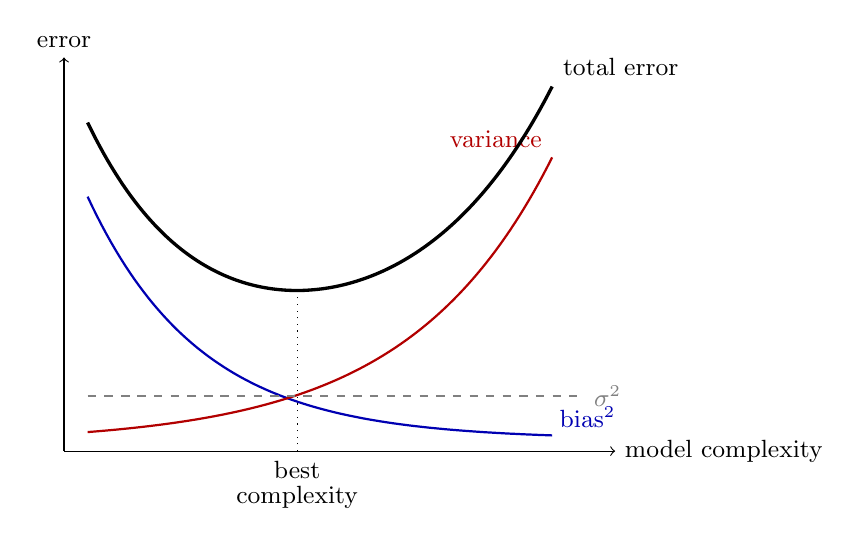
\begin{tikzpicture}[scale=1.0]
    % axes
    \draw[->] (0,0) -- (7,0) node[right] {\small model complexity};
    \draw[->] (0,0) -- (0,5) node[above] {\small error};
    % bias^2 : decreasing
    \draw[thick, blue!70!black, domain=0.3:6.2, samples=100]
        plot (\x, {3.8*exp(-0.7*\x)+0.15}) node[above right=-1pt, blue!70!black] {\small bias$^2$};
    % variance : increasing
    \draw[thick, red!70!black, domain=0.3:6.2, samples=100]
        plot (\x, {0.12*exp(0.55*\x)+0.1}) node[above left] {\small variance};
    % irreducible noise : constant
    \draw[thick, gray, dashed, domain=0.3:6.6]
        plot (\x, {0.7}) node[right, gray] {\small $\sigma^2$};
    % total error : U-shape (sum)
    \draw[very thick, black, domain=0.3:6.2, samples=120]
        plot (\x, {3.8*exp(-0.7*\x)+0.15 + 0.12*exp(0.55*\x)+0.1 + 0.7})
        node[above right] {\small total error};
    % sweet spot (minimum of the total curve, at x = ln(2.66/0.066)/1.25)
    \draw[dotted] (2.96,0) -- (2.96,2.04);
    \node[below] at (2.96,0) {\small \shortstack{best\\complexity}};
\end{tikzpicture}
\end{center}

\paragraph{Link with regularisation.}
This is exactly the knob that ridge regression turns. Increasing the regularisation
strength $\lambda$ shrinks the weights, which makes the predictor less sensitive to
the data (\emph{lower variance}) at the cost of pulling it away from any single
dataset's fit (\emph{higher bias}). Tuning $\lambda$ is therefore a direct way to
navigate the bias-variance tradeoff, and the optimal $\lambda$ is the one balancing
the two.

\begin{remark}[Why ``more of a theorem'']
Nothing in the derivation used the squared loss being applied to a \emph{linear}
model, nor even that $\hat f$ comes from least squares: the decomposition holds for
\emph{any} learning procedure $\mathcal{D} \mapsto \hat f$, as long as the error is
measured in squared loss. This is what makes the bias-variance tradeoff a general
lens rather than a fact about one algorithm.
\end{remark}


\subsection{Working it out for least squares and ridge}
\label{subsec:bv-ridge}

Everything so far has been abstract: bias and variance were defined but never
computed. For the two procedures of \Cref{subsec:ridge} they can be computed exactly,
in a few lines, and the answer is worth the effort: it turns the qualitative U-curve
into a formula, and it delivers one genuinely surprising conclusion.

\paragraph{The setting.}
We simplify in two ways, both standard. First, the design is \emph{fixed}: the inputs
$x_1, \dots, x_n$ are deterministic and only the noise is random, so
\[
y = X w^\star + \varepsilon , \qquad \E[\varepsilon] = 0, \qquad
\E[\varepsilon \varepsilon^\top] = \sigma^2 I_n .
\]
Second, the model is \emph{well specified}: the truth really is linear,
$f^\star(x) = \langle w^\star, x \rangle$ for some $w^\star \in \R^d$. Note the shift
of meaning, which is the usual convention in statistics but worth flagging: in this
subsection $w^\star$ is the \emph{true} parameter, matching the star of $f^\star$,
whereas in \Cref{subsec:ridge} it denoted a minimiser of the empirical risk. Fitted
quantities carry a hat here, as in $\hat w$. We measure the
error \emph{in sample}, that is, averaged over the training inputs themselves:
\[
\mathcal{E}(\hat w) \ \coloneqq \ \frac{1}{n} \sum_{i=1}^n
\E\Big[ \big( \langle \hat w, x_i \rangle - f^\star(x_i) \big)^2 \Big]
\ = \ \frac{1}{n}\, \E \big\Vert X \hat w - X w^\star \big\Vert^2 .
\]
This is the quantity of the theorem above, averaged over $x_0 \in \{x_1, \dots, x_n\}$
and with the constant $\sigma^2$ removed; it splits into bias$^2$ plus variance in
exactly the same way.

\paragraph{Ordinary least squares: no bias, and a variance you can read off.}

\begin{prop}[In-sample error of least squares]
\label{prop:bv-ols}
Assume $\rank(X) = d$, so that $\hat w = (X^\top X)^{-1} X^\top y$ is well defined.
Then $\hat w$ is \emph{unbiased}, $\E[\hat w] = w^\star$, so the bias vanishes at every
point, and
\[
\boxed{\ \mathcal{E}(\hat w) = \underbrace{0}_{\mathrm{bias}^2} \ + \
\underbrace{\frac{\sigma^2 d}{n}}_{\mathrm{variance}} \ } .
\]
\end{prop}

\begin{proof}
Substituting $y = X w^\star + \varepsilon$ into the closed form,
\[
\hat w = (X^\top X)^{-1} X^\top (X w^\star + \varepsilon)
= w^\star + (X^\top X)^{-1} X^\top \varepsilon ,
\]
and taking expectations gives $\E[\hat w] = w^\star$ since $\E[\varepsilon] = 0$.
Hence $X\hat w - X w^\star = \Pi \varepsilon$, where $\Pi \coloneqq X (X^\top X)^{-1}
X^\top$ is the orthogonal projector onto the column space of $X$ (this is the
projection met in the geometric interpretation of least squares). Therefore
\[
\mathcal{E}(\hat w) = \frac1n \E \Vert \Pi \varepsilon \Vert^2
= \frac1n \E\big[ \varepsilon^\top \Pi \varepsilon \big]
= \frac{\sigma^2}{n} \tr(\Pi) = \frac{\sigma^2 d}{n} ,
\]
using $\Pi^\top \Pi = \Pi$ and $\tr(\Pi) = \rank(X) = d$ for a projector.
\end{proof}

This one formula contains most of the intuition of the whole chapter. The error is
$\sigma^2 d / n$: it grows \emph{linearly with the number of features} and decays like
$1/n$. Each extra feature buys one more direction in which the estimator can chase the
noise, at a cost of exactly $\sigma^2/n$, and it is worth paying only if that feature
removes at least as much bias. This is the bias-variance tradeoff, made arithmetic.
Notice also what happens as $d$ approaches $n$: the error tends to $\sigma^2$, as large
as the noise itself, which is the first hint of the spike we will meet in
\Cref{subsec:double-descent}.

\paragraph{Ridge: paying bias to buy variance.}
For ridge nothing is unbiased any more, and the clean way to see both terms at once is
to diagonalise. Let
\[
X^\top X = \sum_{j=1}^d \mu_j\, u_j u_j^\top
\]
be an eigendecomposition, with eigenvalues $\mu_1, \dots, \mu_d \geq 0$ and
orthonormal eigenvectors $u_1, \dots, u_d$, and write $c_j \coloneqq \langle u_j,
w^\star \rangle$ for the coordinates of the truth in that basis. (In this subsection we
call the eigenvalues $\mu_j$, and not $\lambda_j$ as one normally would, because
$\lambda$ is already the regularisation strength. In \Cref{subsec:pca}, where no
regularisation appears, they go back to being $\lambda_j$.)

\begin{prop}[In-sample error of ridge]
\label{prop:bv-ridge}
For $\hat w_\lambda = (X^\top X + n\lambda I)^{-1} X^\top y$ and any $\lambda > 0$,
\[
\mathcal{E}(\hat w_\lambda)
= \underbrace{n \lambda^2 \sum_{j=1}^d \frac{\mu_j\, c_j^2}{(\mu_j + n\lambda)^2}}_{\mathrm{bias}^2(\lambda)}
\ + \ \underbrace{\frac{\sigma^2}{n} \sum_{j=1}^d \frac{\mu_j^2}{(\mu_j + n\lambda)^2}}_{\mathrm{variance}(\lambda)} .
\]
The first sum increases from $0$ to $\tfrac1n \Vert X w^\star\Vert^2$ as $\lambda$ goes
from $0$ to $\infty$; the second decreases from $\sigma^2 d / n$ to $0$.
\end{prop}

\begin{proof}
Write $M_\lambda \coloneqq (X^\top X + n \lambda I)^{-1}$, so that $\hat w_\lambda =
M_\lambda X^\top y = M_\lambda X^\top X w^\star + M_\lambda X^\top \varepsilon$. Taking
expectations and using $M_\lambda X^\top X = I - n\lambda M_\lambda$,
\[
\E[\hat w_\lambda] - w^\star = - n \lambda\, M_\lambda w^\star ,
\qquad
\hat w_\lambda - \E[\hat w_\lambda] = M_\lambda X^\top \varepsilon .
\]
The first identity gives the bias term: since $M_\lambda w^\star = \sum_j c_j (\mu_j +
n\lambda)^{-1} u_j$,
\[
\mathrm{bias}^2 = \frac1n \big\Vert X \cdot n\lambda M_\lambda w^\star \big\Vert^2
= n \lambda^2 \, (M_\lambda w^\star)^\top X^\top X\, (M_\lambda w^\star)
= n\lambda^2 \sum_{j=1}^d \frac{\mu_j c_j^2}{(\mu_j + n\lambda)^2} .
\]
The second gives the variance term:
\[
\mathrm{variance} = \frac1n \E \big\Vert X M_\lambda X^\top \varepsilon \big\Vert^2
= \frac{\sigma^2}{n} \tr\big( M_\lambda X^\top X M_\lambda X^\top X \big)
= \frac{\sigma^2}{n} \sum_{j=1}^d \frac{\mu_j^2}{(\mu_j + n\lambda)^2} .
\]
Both monotonicity statements are read off term by term, and the stated limits follow
from $\sum_j \mu_j c_j^2 = \Vert X w^\star \Vert^2$ and, when $\rank(X) = d$, from
$\mu_j > 0$ for every $j$.
\end{proof}

The two sums are the two arms of the U-curve, now completely explicit, and one sees
precisely how $\lambda$ trades them off: every eigendirection $j$ is shrunk by the
factor $\mu_j / (\mu_j + n\lambda) \in (0,1)$, which is close to $1$ for the directions
the data determines well ($\mu_j \gg n\lambda$, barely touched) and close to $0$ for
those it determines badly ($\mu_j \ll n\lambda$, essentially switched off). Ridge does
not shrink uniformly: it discards exactly the directions in which the data is
uninformative, which is precisely what the minimum-norm rule was doing implicitly in
\Cref{subsec:overparam}.

\paragraph{The surprise: $\lambda = 0$ is never optimal.}

\begin{corollary}[A little regularisation always helps]
\label{cor:ridge-beats-ols}
Assume $\rank(X) = d$ and $\sigma^2 > 0$. Then, as a function of $\lambda$, the
in-sample error satisfies
\[
\frac{\mathrm{d}}{\mathrm{d}\lambda} \, \mathcal{E}(\hat w_\lambda) \Big|_{\lambda = 0}
= - 2 \sigma^2 \sum_{j=1}^d \frac{1}{\mu_j} \ < \ 0 .
\]
In particular there exists $\lambda > 0$ with $\mathcal{E}(\hat w_\lambda) <
\mathcal{E}(\hat w_0) = \sigma^2 d / n$: \emph{some} amount of ridge regularisation
strictly beats ordinary least squares, whatever the data and whatever the truth
$w^\star$.
\end{corollary}

\begin{proof}
Set $u = n\lambda$. Near $u = 0$ the bias term is $\tfrac{u^2}{n}\sum_j \mu_j c_j^2
\mu_j^{-2} + O(u^3)$, so it is $O(u^2)$ and its derivative at $u = 0$ vanishes: the
bias costs nothing \emph{to first order}. The variance term, on the other hand, has
derivative $\tfrac{\sigma^2}{n} \sum_j (-2)\mu_j^2 (\mu_j + u)^{-3}$, equal to
$-\tfrac{2\sigma^2}{n}\sum_j \mu_j^{-1}$ at $u = 0$: it decreases at a strictly
positive rate. Multiplying by $\mathrm{d}u/\mathrm{d}\lambda = n$ gives the claim.
\end{proof}

This is worth pausing on, because it is not what one expects. Least squares is
unbiased, and unbiasedness sounds like a virtue; the corollary says it is the wrong
thing to optimise. Starting from $\lambda = 0$, a small penalty buys a first-order
reduction in variance for only a second-order increase in bias, so the trade is always
favourable at the start. The size of the gain is governed by $\sum_j 1/\mu_j$, which is
enormous exactly when $X^\top X$ has small eigenvalues, i.e.\ when the features are
nearly collinear and the least-squares fit is unstable. That is the regime where
practitioners reach for ridge, and this is the calculation that justifies them.

\begin{remark}[What the calculation does \emph{not} say]
Note that \Cref{cor:ridge-beats-ols} guarantees the existence of a good $\lambda$; it
does not tell us its value, which depends on the unknowns $\sigma^2$ and $w^\star$.
Choosing $\lambda$ in practice is done by cross-validation (\Cref{subsec:cv}), not by
this formula. What the formula gives is the reassurance that the search is not in vain,
and an understanding of when it will pay off most.
\end{remark}


\subsection{A puzzle: what about over-parametrised models?}
\label{subsec:double-descent}

At this point you should be suspicious. In \Cref{subsec:overparam} we insisted that
the regime $d > n$ is ``the rule rather than the exception in modern machine
learning'': the networks that work best in practice have far more parameters than
training samples, and they interpolate their training data exactly. But the U-curve
we have just drawn says that such models sit at the far right of the complexity axis,
drowning in variance, and should therefore be catastrophic. They are not. What is
going on?

The resolution is that \emph{``complexity'' was never the same thing as ``number of
parameters''}. The horizontal axis of the U-curve measures how much a procedure
can wobble when the data changes, and the derivation above bounds nothing about how
that relates to $d$. What the bias-variance theorem decomposes is the error of a
\emph{learning procedure}, dataset $\mapsto$ predictor, and adding parameters changes
that procedure in two ways at once:
\begin{itemize}
    \item it enlarges the function class $\F$, which is the effect the U-curve has in
    mind, and which does push the variance up;
    \item but once $d > n$ it also makes the minimiser \emph{non-unique}, and the
    procedure is then defined only by the extra rule we use to choose among the
    interpolants. In our case that rule is the minimum-norm one, reached either
    explicitly (ridge, as $\lambda \to 0^+$) or implicitly (gradient descent from
    $w_0 = 0$).
\end{itemize}
That second effect works in the \emph{opposite} direction. The more features we add
beyond $n$, the larger the space $\ker(X)$ of directions the data says nothing about,
and the harder the minimum-norm rule is pushing back towards $0$ along all of them.
Adding parameters past the interpolation threshold therefore keeps enriching the
class while \emph{also} strengthening the implicit regularisation, and the variance
can start going down again.

The empirical shape that results is called \emph{double descent}: as $d$ grows the
test error first traces the classical U-curve, then \emph{spikes} around the
interpolation threshold $d \approx n$ (where $X$ is barely invertible, $\Vert
w^\dagger \Vert$ blows up, and the fit is maximally unstable), and then descends a
\emph{second} time in the over-parametrised regime $d \gg n$, sometimes going below
the best error of the first descent.

\begin{remark}[The moral]
The bias-variance decomposition is a theorem and remains exactly true in the
over-parametrised regime: the test error is still noise plus bias$^2$ plus variance.
What is \emph{not} a theorem, and what modern practice violates, is the folklore that
variance increases monotonically with the number of parameters. This is why the
implicit bias of gradient descent, proved in \Cref{subsec:gd}, is not a curiosity: in
the over-parametrised regime it \emph{is} the regularisation, and it is what decides
whether a model that interpolates its training data generalises or not.
\end{remark}


\subsection{Estimating the test error: validation and cross-validation}
\label{subsec:cv}

Everything above is about a quantity, the test error, that we have never explained
how to \emph{compute}. This is not a detail: the whole discussion tells us to pick the
model complexity, or the ridge parameter $\lambda$, at the bottom of the U-curve, and
we cannot do that without a number to minimise. The decomposition itself is of no help
here, since $f^\star$ and $\sigma^2$ are unknown. What follows is how it is done in
practice, and it is the single most used recipe in all of machine learning.

\paragraph{Why the training error will not do.}
The obvious candidate, the empirical risk $L(\hat w)$ on the data we fitted on, is
useless, and the two extremes above show exactly why: it can be driven to zero by a
procedure that generalises terribly. The reason is that $\hat w$ was \emph{chosen
using} those very points, so the residuals on them are not representative. Any
estimate of the test error must be computed on data the fitting procedure has
not seen.

\paragraph{The train / validation / test split.}
The remedy is to spend our $n$ samples on three different jobs, splitting them at
random into three disjoint parts.
\begin{itemize}
    \item The \emph{training set} (say $60\%$) is used to fit $\hat w$, for each
    candidate value of the quantity we are trying to choose (the polynomial degree
    $k$, the ridge parameter $\lambda$, \dots). Such a quantity, which is not fitted by
    the optimiser but selected from outside, is called a \emph{hyperparameter}.
    \item The \emph{validation set} (say $20\%$) is used to \emph{compare} those
    fitted models: we evaluate the squared error of each on it and keep the
    hyperparameter achieving the smallest one. This is our estimate of the U-curve,
    and its minimiser is our estimate of the best complexity.
    \item The \emph{test set} (say $20\%$) is locked away until the very end and used
    exactly once, to report the error of the final model.
\end{itemize}

\begin{remark}[Why a third set is needed]
The last point is the one most often skipped, and it matters. Once we have minimised
the validation error over, say, twenty values of $\lambda$, the winning value was
selected \emph{because} it did well on the validation set, and part of why it did well
is luck specific to those points. The validation error of the winner is therefore
optimistically biased, for exactly the same reason the training error was: it is the
minimum over many noisy quantities. The test set is untouched by any choice we made,
so it gives an honest number. A useful way to put it: the validation set is used to
\emph{choose}, the test set only to \emph{report}.
\end{remark}

\paragraph{$K$-fold cross-validation.}
A single validation set is wasteful when $n$ is small: we throw away $20\%$ of the
data when fitting, and the resulting estimate is itself noisy, since it depends on
which points happened to land in the validation part. \emph{Cross-validation} fixes
both problems by rotating the role of the validation set. Split the training data into
$K$ disjoint blocks (\emph{folds}) $I_1, \dots, I_K$ of roughly equal size. Then, for
each fold $k = 1, \dots, K$:
\begin{itemize}
    \item fit the model on everything \emph{except} $I_k$, giving a parameter
    $\hat w^{(-k)}$;
    \item evaluate the error on the held-out fold $I_k$, which was not used for that
    fit,
    \[
    e_k = \frac{1}{|I_k|} \sum_{i \in I_k}
    \big( \langle \hat w^{(-k)}, x_i \rangle - y_i \big)^2 .
    \]
\end{itemize}
The cross-validation score is the average $\mathrm{CV} = \tfrac{1}{K} \sum_{k=1}^K
e_k$, and we choose the hyperparameter minimising it. Every point is used for fitting
in $K-1$ of the folds and for evaluation in exactly one, so no data is wasted and the
averaging over $K$ folds reduces the variance of the estimate. The price is that we
now fit $K$ models per hyperparameter value instead of one.

Typical choices are $K = 5$ or $K = 10$. The extreme case $K = n$, in which each fold
is a single point, is called \emph{leave-one-out} cross-validation: it uses the data
maximally but requires $n$ fits, which is usually prohibitive.

\begin{remark}[Two traps]
\emph{Split before you preprocess.} Any quantity estimated from the data, in
particular the feature means and standard deviations used for standardisation, must be
computed on the training part only and then applied to the validation and test parts.
Standardising the full dataset first lets information about the held-out points leak
into the fit, and the resulting estimate is again optimistic; see
\Cref{subsec:standardise}. \emph{Split
respecting the structure of the data.} The reasoning above assumes the samples are
independent. For time series, or when several samples come from the same patient or
the same user, a uniformly random split puts near-duplicates on both sides and makes
the estimate meaningless; one splits by time, or by patient, instead.
\end{remark}

\begin{exercise}[$\star$]
Take the polynomial model of degree $k$ on a small dataset. Plot, as functions of $k$,
the training error and the $5$-fold cross-validation error on the same axes. Which one
is U-shaped? Which one is monotone, and in which direction? Compare with the figure
above.
\end{exercise}
